\chapter{Introdução}



\chapter{Descrição Teórica do Sistema}


Para se projetar um sedimentador industrial é preciso determinar a área e a altura deste, com base no valor de concentração da alimentação e a concentração desejada na saída do sedimentador. Para isso, é necessário realizar testes de proveta para determinar alguns parâmetros em escala de laboratório.

Durante os testes de proveta, utiliza-se uma suspensão com as mesmas condições de temperatura e pH que são encontradas nos processo industrial. O teste de proveta permite obter a curva de posição da interface em função do tempo. A partir dessa curva, são obtidos parâmetros \emph{cinéticos} que permitem estimar a área e altura do sedimentador industrial.


\section{Etapas de Sedimentação e o teste da proveta}

Durante o processo de sedimentação, quatro zonas são formadas e nos testes de proveta realizados em escala de bancada, elas não são muito bem definidas.A fim de entender melhor como ocorre o mecanismo da sedimentação e como ela ocorre ao passar do tempo, pode-se analisar a Figura \ref{etapasprov}.


\begin{figure}[H]
	\begin{center}
		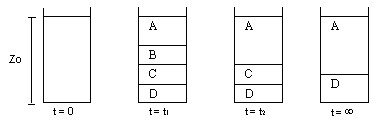
\includegraphics[scale=.8, trim={0 0 0 0}]{figuras/ladeq/sedi/proveta}
		%\vspace{-20pt}
		\caption{Mecanismo de sedimentação.}
		\label{etapasprov}
	\end{center}
\end{figure}


No início da decantação (t = 0), a suspensão encontra-se a uma altura $ Z_{0} $ e sua concentração é uniforme. Pouco tempo depois (t = $ t_{1} $ ) é possível distinguir quatro zonas distintas. São elas:


\begin{itemize}
\item A - Líquido Clarificado: esta camada pode ficar turva durante certo tempo devido à presença de partículas mais finas que permanecem em suspensão;
\item B - Região de Concentração constante ou concentração inicial: tem-se a sedimentação livre, isto é, desconsideram-se os efeitos de concentração, como se as partículas sedimentassem de forma isolada;
\item C - Região de Concentração Variável: nesta região a concentração da suspensão aumenta gradativamente, variando da concentração inicial até a concentração da suspensão espessada, e já se observa o efeito da concentração;
\item D - Região de Lama (compactação): à medida que ocorre a sedimentação a espessura desta região aumenta.  
\end{itemize}

À medida que a sedimentação ocorre, as regiões A e D tornam-se mais importantes e as regiões B e C tendem a desaparecer. 
A velocidade de sedimentação aumenta na região de clarificado (aceleração) e, a partir deste ponto, permanece constante até o final da região B. A velocidade tende a diminuir (desaceleração) em seguida até alcançar o ponto crítico de sedimentação, momento em que a região B desaparece \citep{macabe}.

Esse comportamento pode ser observado na Figura \ref{sedimentaP}.


\begin{figure}[H]
	\begin{center}
		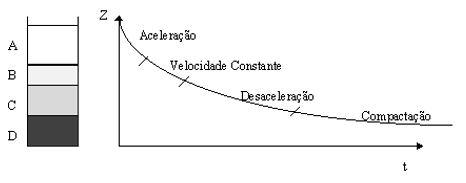
\includegraphics[scale=.8,trim={0 0 0 0}]{figuras/ladeq/sedi/graphProv}
		%\vspace{-20pt}
		\caption{Processo de Sedimentação.}
		\label{sedimentaP}
	\end{center}
\end{figure}

O ponto crítico pode ser determinado, pois enquanto a região B, de concentração igual à inicial, ainda existe, a velocidade de sedimentação é constante e, assim, a variação da altura da interface com o tempo é linear. Porém, ao B desaparecer, a velocidade de sedimentação começa a variar, devido ao fato da concentração também ser variável. Conforme a concentração aumentar, a velocidade de sedimentação diminui, como ilustrado na Figura \ref{linearReg}.


\begin{figure}[H]
	\begin{center}
		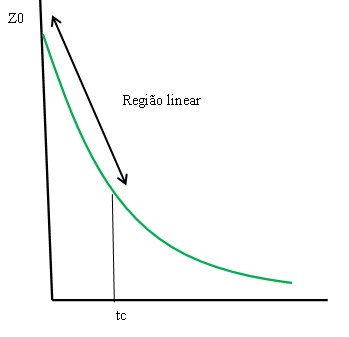
\includegraphics[scale=.5,trim={0 0 0 0}]{figuras/ladeq/sedi/graphProv2}
		%\vspace{-20pt}
		\caption{Determinação gráfica do tempo crítico (tC).}
		\label{linearReg}
	\end{center}
\end{figure}

\section{Balanço de Massa}

Um sedimentador, com suas respectivas correntes e concentrações, é representado no esquema da Figura \ref{esquema}.

\begin{figure}[H]
	\begin{center}
		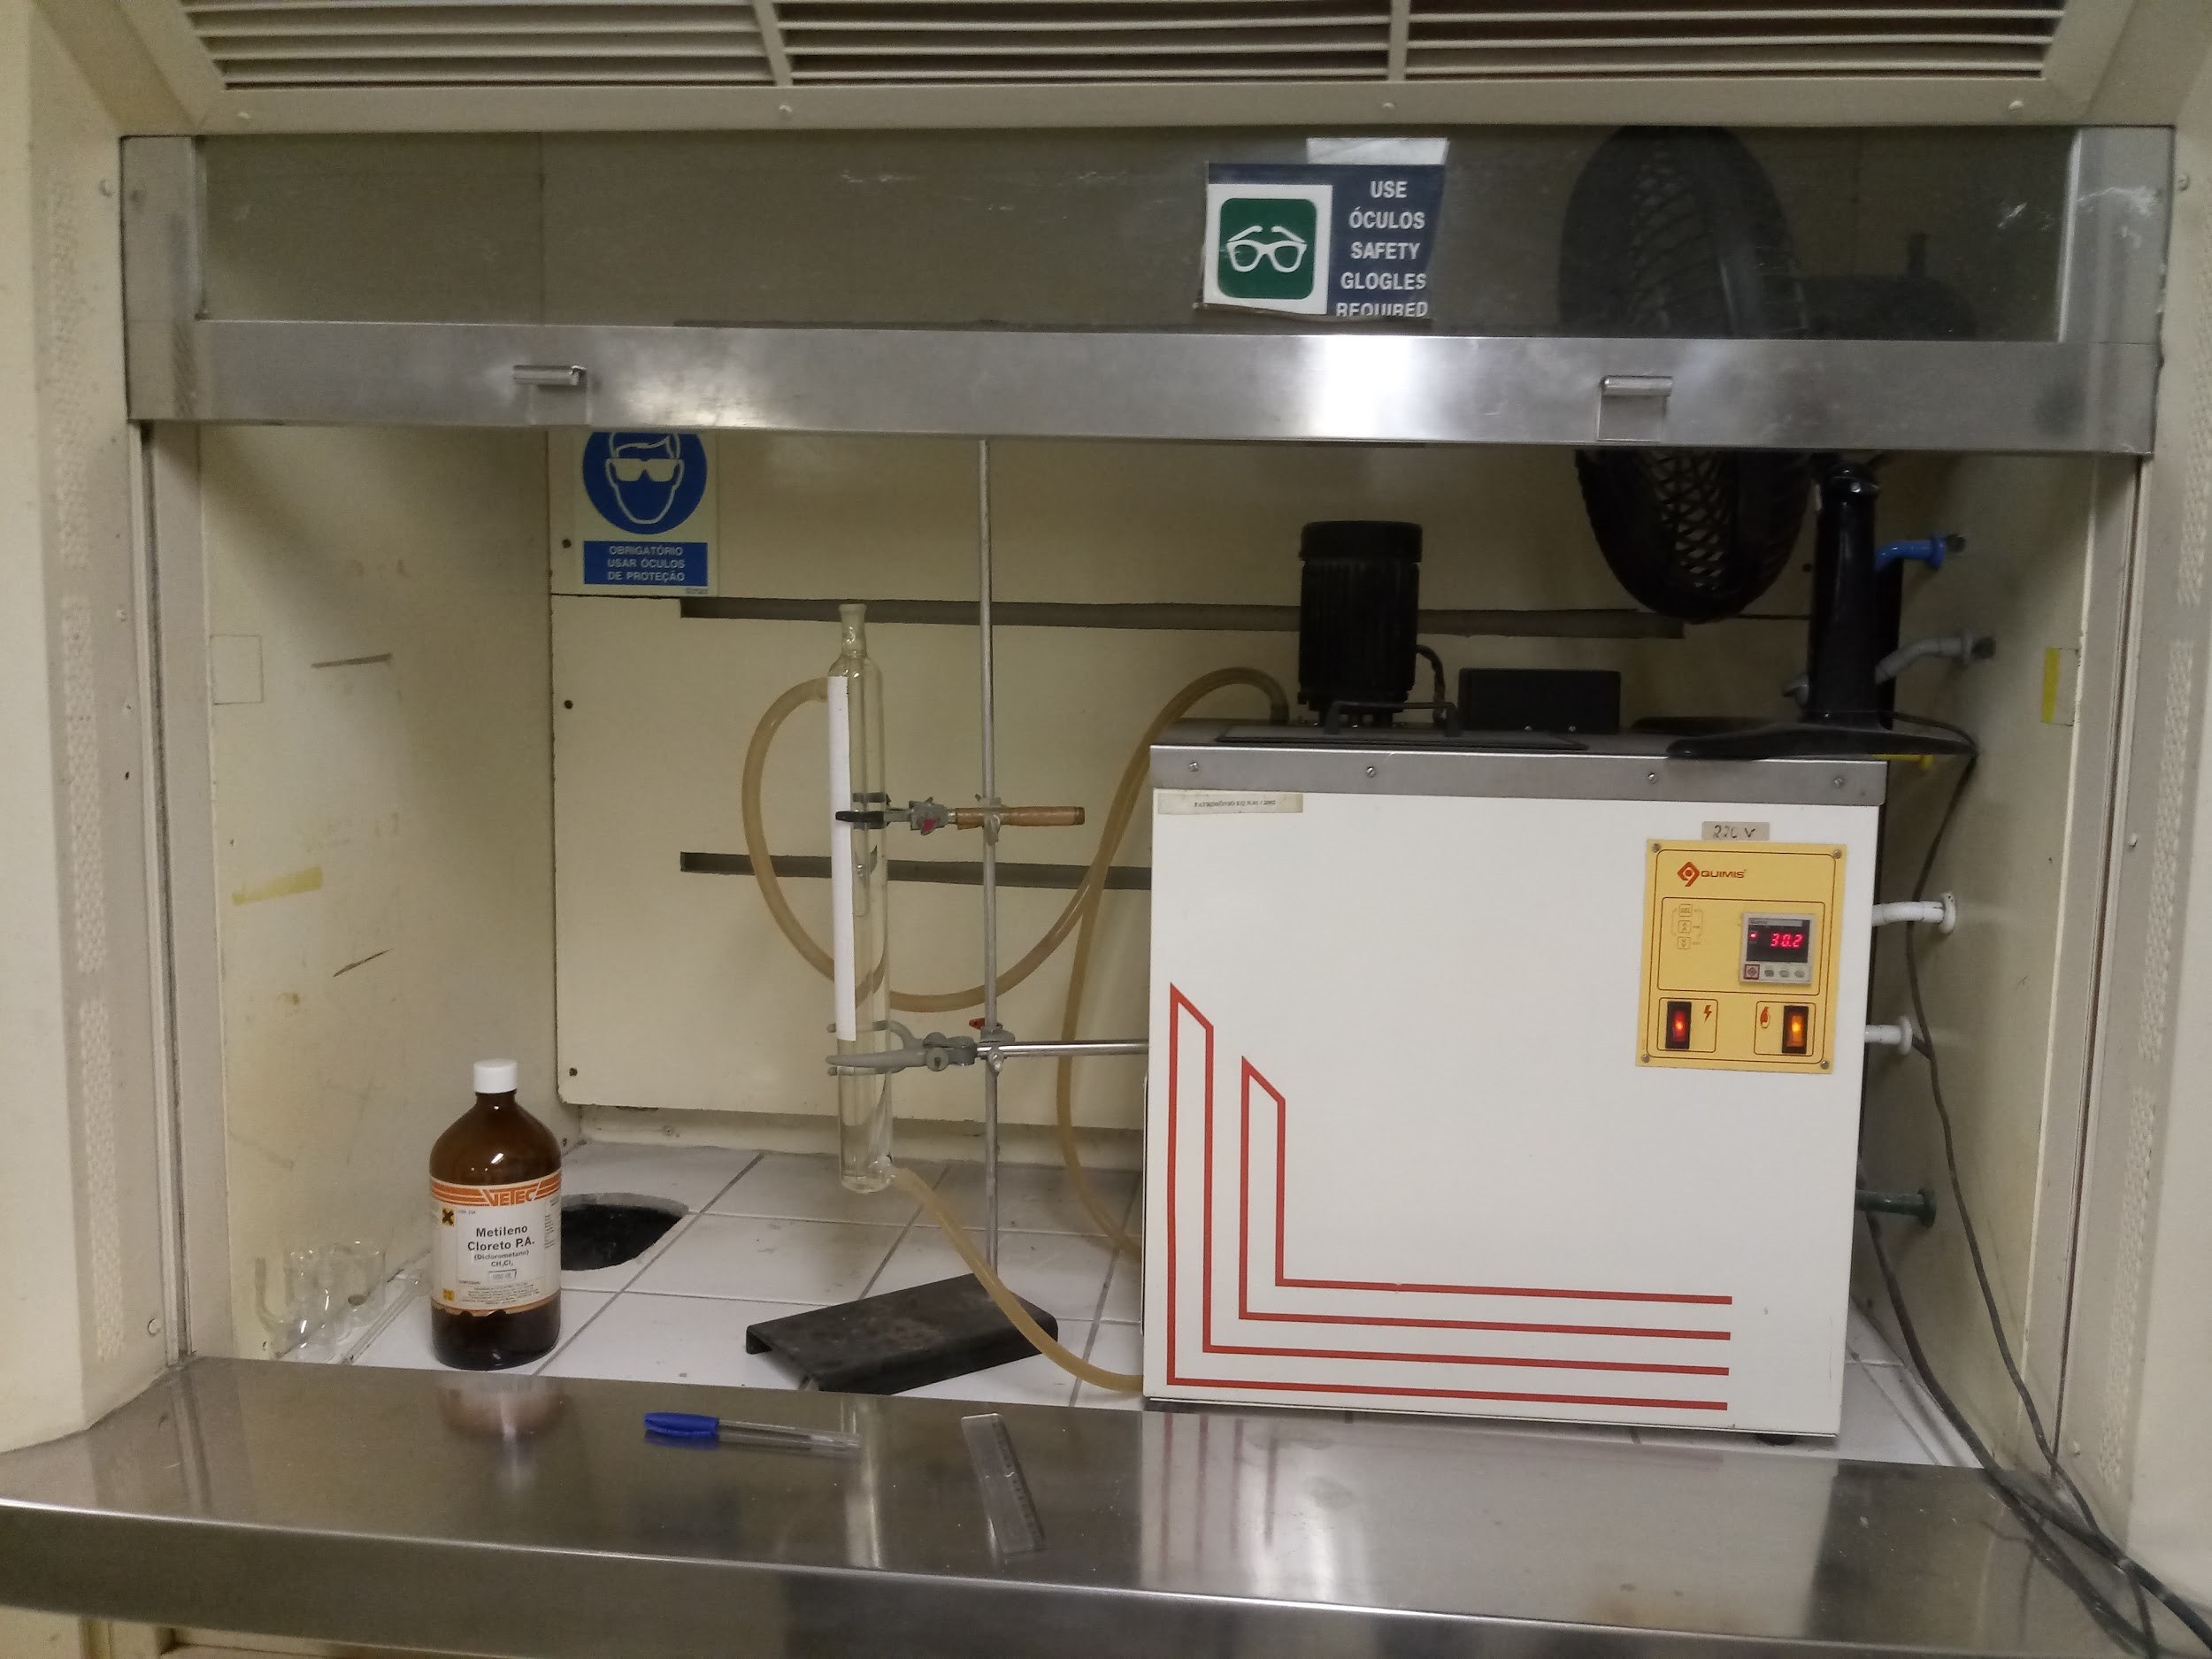
\includegraphics[scale=.5,trim={0 0 0 0}]{figuras/ladeq/sedi/aparato}
		%\vspace{-20pt}
		\caption{Esquema de um sedimentador e suas variáveis.}
		\label{esquema}
	\end{center}
\end{figure}

Em que:

\begin{itemize}
\item Q – Vazão da alimentação
\item $ C_{v} $ – Concentração volumétrica de sólidos na alimentação
\item $ Q_{o} $ – Vazão volumétrica do overflow (líquido clarificado)
\item $ C_{vo} $ – Concentração volumétrica de sólidos no overflow
\item $ Q_{u} $ – Vazão volumétrica do underflow (sólidos concentrados, “lama”)
\item $ C_{vu }$ – Concentração volumétrica de sólidos no underflow
\item $ Q_{a} $ – Vazão volumétrica de líquido límpido no nível L em sentido ascendente
\item $ Q_{L} $ – Vazão volumétrica no nível L em sentido descendente
\item $ C_{vL} $ – Concentração de sólidos no nível L em sentido descendente
\end{itemize}



Para se iniciar o balanço de massa, considera-se que a concentração de sólidos na corrente de líquido clarificado é igual à zero. Logo, a vazão ascendente consiste apenas de líquido clarificado $ (C_{V0} = 0) $. Portanto, temos o seguinte balanço de massa para os sólidos:

\begin{equation}\label{key}
\rho s \times Q \times C v=\rho s \times Q u \times C v u=\rho s \times Q_{L} \times C v L
\end{equation}


Sendo $\rho_{S}$ a densidade das partículas sólidas. Portanto:

\begin{equation}\label{key}
\mathrm{Qu}=\mathrm{Q} \times \frac{\mathrm{Cv}}{\mathrm{Cvu}}
\end{equation}

Já para o líquido, temos o seguinte balanço de massa, no nível L:

\begin{equation}\label{key}
\rho \times \mathrm{Q}_{L} \times(1-\mathrm{CvL})=\rho \times \mathrm{Qa}+\rho \times \mathrm{Qu} \times(1-\mathrm{Cvu})
\end{equation}

Sendo $\rho$ a densidade do líquido. 
Assim,

\begin{equation}\label{key}
\mathrm{Qu}=\frac{\mathrm{Q}_{L} \times \mathrm{CvL}}{\mathrm{Cvu}}
\end{equation}

\begin{equation}\label{key}
Q_{L} \times(1-C v L)=Q a+\frac{Q_{L} \times C_{V L}}{C v u} \times(1-C v u)
\end{equation}

\begin{equation}\label{key}
\mathrm{Qa}=\mathrm{Q}_{L}-\mathrm{Q}_{L} \times \mathrm{CvL}-\frac{\mathrm{Q}_{L} \times \mathrm{CvL}}{\mathrm{Cvu}}+\mathrm{Q}_{L} \times \mathrm{CvL}
\end{equation}

\begin{equation}\label{key}
\mathrm{Q}_{L} \times \mathrm{CvL}=\mathrm{Q} \times \mathrm{Cv}
\end{equation}

\begin{equation}\label{key}
\mathrm{Qa}=\mathrm{Q}_{\mathrm{L}}-\frac{\mathrm{Q}_{L} \times \mathrm{CVL}}{\mathrm{Cvu}}=\mathrm{Q}_{L} \times \operatorname{CvL} \times\left(\frac{1}{\mathrm{CVL}}-\frac{1}{\mathrm{Cvu}}\right)
\end{equation}

\begin{equation}\label{key}
\mathrm{Qa}=\mathrm{Q} \times \mathrm{Cv} \times\left(\frac{1}{\mathrm{CvL}}-\frac{1}{\mathrm{Cvu}}\right)
\end{equation}

\begin{equation}\label{key}
\frac{\mathrm{Qa}}{\mathrm{A}}=\frac{\mathrm{Q} \times \mathrm{Cv}}{\mathrm{A}} \times\left(\frac{1}{\mathrm{CvL}}-\frac{1}{\mathrm{Cvu}}\right)
\end{equation}

A hipótese do método de Coe e Clevenger se baseia na sedimentação das partículas. Este método foi o primeiro a ser desenvolvido e é a fundamentação dos demais.Ele parte da ideia de que todas as partículas alimentadas devem seguir para zona de espessado. Caso isto não ocorra, acarretará no acúmulo de partículas, devido ao arraste, numa dada região chamada de zona limite.

Para tanto, tomando como base que $ C_{V0} = 0 $, a velocidade de ascensão do líquido deve ser menor que a velocidade de sedimentação das partículas, evitando, assim, que elas sejam arrastadas no sentido ascendente. Portanto, deve-se ter:



\begin{equation}\label{key}
\frac{\mathrm{Qa}}{\mathrm{A}} \leq \mathrm{v}
\end{equation}

Onde: $ \frac{Qa}{A} = $ velocidade de ascensão do fluido e v = velocidade de sedimentação das partículas.

No limite, tem-se:

\begin{equation}\label{key}
\frac{\mathrm{Qa}}{\mathrm{A}}=\mathrm{v}
\end{equation}

Assim:

\begin{equation}\label{key}
\frac{\mathrm{Q} \times \mathrm{Cv}}{\mathrm{A}} \times\left(\frac{1}{\mathrm{CvL}}-\frac{1}{\mathrm{Cvu}}\right)=\mathrm{v}
\end{equation}

Chegamos, então, à fórmula da área mínima:

\begin{equation}\label{key}
\mathrm{A}=\frac{\mathrm{Q} \times \mathrm{C} \mathrm{v}}{\mathrm{v}} \times\left(\frac{\mathrm{1}}{\mathrm{C} \mathrm{v} \mathrm{L}}-\frac{\mathrm{1}}{\mathrm{C} \mathrm{v} \mathrm{u}}\right)
\end{equation}


\section{Método de Kynch}

Kynch desenvolveu um método de dimensionamento de sedimentadores que necessita de apenas um ensaio experimental, diferentemente do método de Cloe e Clevenger, que exige inúmeros experimentos. 

O ensaio é iniciado com uma concentração uniforme $ C_{0} $. Supondo que, numa determinada seção do decantador, onde a concentração possui um valor C, a capacidade do equipamento passa por um mínimo e chega até um máximo quando o sistema está em operação, é nesse momento que uma zona característica começará a se formar nessa seção \citep{foust}. 

Se a seção transversal S for insuficiente,ocorrerá acúmulo de sólidos e a zona limite será deslocada para mais perto da saída de clarificado. Mas se a área for suficiente, em regime permanente, os sólidos que entram no sistema também saem.


O procedimento proposto por Kynch requer apenas um ensaio de decantação que forneça a curva de decantação (Z em função de t), através do qual se traçam tangentes em diversos pontos da curva e determinam-se os valores de t, Z e $ Z_{i} $. Com esses valores (t, Z e $ Z_{i} $), utiliza-se a expressão do método de Coe e Clevenger para obter as áreas da seção transversal.

O valor máximo de área obtida corresponderá à área mínima que o decantador poderá ter.

O método gráfico pode ser verificado na Figura \ref{met}.

\begin{figure}[H]
	\begin{center}
		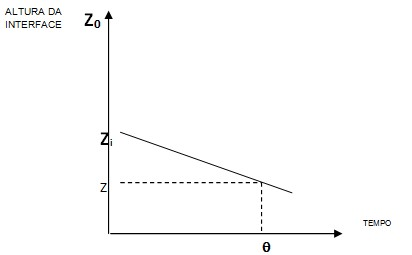
\includegraphics[scale=.5,trim={0 0 0 0}]{figuras/ladeq/sedi/graphKynch}
		%\vspace{-20pt}
		\caption{Exemplo de resultado do método de Kynch.}
		\label{met}
	\end{center}
\end{figure}


A reta tangente pode ser obtida após o cálculo de cada derivada, para cada altura da interface de sedimentação z, correspondente a um tempo de sedimentação t, utilizando as fórmulas a seguir:

\begin{equation}\label{key}
z=\frac{\mathrm{d} z}{\mathrm{dt}} \mathrm{t}+\mathrm{zi} \quad \quad \mathrm{zi}=z-\frac{\mathrm{d} z}{\mathrm{dt}} \mathrm{t}
\end{equation}

Assim, a concentração de sólidos em um nível L qualquer $ C_{vL} $ pode ser calculada, a partir dos valores de $ z_{i} $ correspondentes a cada altura da interface z, através da seguinte relação:

\begin{equation}\label{key}
\mathrm{C_{vL}}=\mathrm{C_{v}} \times \frac{\mathrm{z} _{0}}{\mathrm{z_{i}}}
\end{equation}

Finalmente, calcula-se a área mínima do sedimentador pela equação obtida pelo balanço de massa realizado acima:

\begin{equation}\label{key}
\operatorname{A_{min}}=\frac{\mathrm{Q} \times \mathrm{C_{v}}}{\mathrm{v}} \times\left(\frac{1}{\mathrm{C_{vL}}}-\frac{1}{\mathrm{C_{vU}}}\right)
\end{equation}

No final do experimento, tem-se um conjunto de áreas mínimas calculadas, que podem ser organizadas em uma tabela como a representada abaixo:

	

\begin{table}[H]
	\centering
	\begin{tabular}{|l|l|l|l|l|l|}
		\hline
		\textbf{t} & \textbf{z} & $ \mathbf{\left( \dfrac{d z}{dt}  \right)} $ & \textbf{zi} & $ \mathbf{C_{vL}} $ & \textbf{A} \\ \hline
		t1 & z1 & $ \left ( \dfrac{d z}{dt}\right )_{1} $ & zi1 & CvL1 & A1 \\ \hline
		t2 & z2 & $ \left ( \dfrac{d z}{dt} \right )_{2} $ & zi2 & CvL2 & A2 \\ \hline
		... & ... & ... & ... & ... & ... \\ \hline
		tn & zn & $ \left ( \dfrac{d z}{dt}\right )_{n} $ & zin & CvLn & An \\ \hline
	\end{tabular}
	\caption{Organização dos dados no método de Kynch.}
	\label{kynch}
\end{table}


Dentre todas as áreas mínimas calculadas pelo método de Kynch, a de maior valor deve ser utilizada como base de cálculo da área de projeto.


\section{Método de Biscaia Jr.}

Esse método é relativamente mais simples do que o método de Kynch. No método de Biscaia Jr., assume-se que a curva da altura da interface em função do tempo pode ser representada por uma função composta, sendo a primeira parte da curva linear e a segunda exponencial. 

$ Z_{\text{mín}} $ tem seu valor determinado a partir da seguinte relação:

\begin{equation}\label{key}
Z_{\min }=z_{0} * \frac{\mathrm{CvO}}{\mathrm{Cvu}}
\end{equation}

E com o valor de $ z_{\text{mín }}$, através do gráfico da Figura \ref{tabqua1}, obtém-se o valor de $ t_{\text{mín}} $.

\begin{figure}[H]
	\begin{center}
		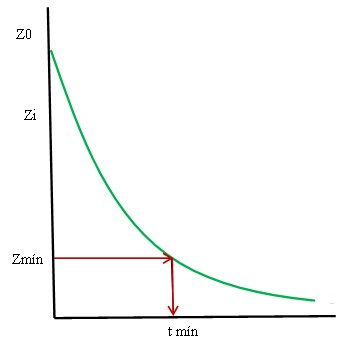
\includegraphics[scale=.5,trim={0 0 0 0}]{figuras/ladeq/sedi/graphBiscaia}
		%\vspace{-20pt}
		\caption{Representação gráfica do método de Biscaia Jr.}
		\label{tabqua1}
	\end{center}
\end{figure}


Com o valor detmín obtido, pode-se então determinar $ A_{\text{mín}} $:

\begin{equation}\label{key}
\operatorname{A_{\text{mín}}}=Q \times \frac{t_{\text{mín}}}{z_{0}}
\end{equation}


\section{Fatores de Correção}

A área determinada por ambos os métodos é a área mínima que o sedimentador deve ter para que se tenha a sedimentação desejada. Porém, é necessário o ajuste de alguns parâmetros para reproduzir as condições operacionais de um sedimentador industrial mais fielmente.


\begin{equation}\label{key}
A_{proj}=\operatorname{A_{\text{mín}}} \times \mathrm{f}_{1} \times \mathrm{f}_{2}
\end{equation}

O fator $ f_{1}  $considera efeitos de pH, temperatura, diâmetro dos flocos e concentração das partículas. Esse fator é especialmente importante em locais onde há grande variação de temperatura.

\begin{equation}\label{key}
1,10 \leq f_{1} \leq 1,25
\end{equation}


Já o fator $ f_{2} $ é função do diâmetro das partículas e considera a turbulência causada pela alimentação da suspensão no sedimentador. Como a velocidade nos tubos de alimentação é muito maior que a velocidade dentro do sedimentador, há geração de uma zona de turbulência na região de alimentação, dificultando a sedimentação. O fator de segurança visa amortecer o efeito da zona de turbulência através do aumento do diâmetro.

\begin{equation}\label{key}
1,10 \mathrm{m}<\mathrm{D}_{\mathrm{min}}<1,25 \mathrm{m} \quad 1,2 \leq \mathrm{f}_{2} \leq 1,5
\end{equation}

\begin{equation}\label{key}
D_{\min } \leq 5 \mathrm{m} \quad \mathrm{f}_{2}=1,5
\end{equation}

\begin{equation}\label{key}
\mathrm{D}_{\mathrm{min}} \geq 30 \mathrm{m} \quad \mathrm{f}_{2}=1,2
\end{equation}


\chapter{Objetivo}


O experimento tem como objetivo determinar o dimensionamento de um sedimentador a partir dos dados coletados em um teste de proveta para a suspensão de $ CaCO_{3} $, utilizando os métodos de Kynch e Biscaia Jr. e fazer comparações com os valores obtidos.

O sedimentador industrial deverá operar com uma suspensão de carbonato de cálcio, de aproximadamente 3\% em peso de $ CaCO_{3} $, para obtenção de uma lama de concentração de sólidos 2 vezes superior à da alimentação.
\\


\chapter{Materiais e Métodos}

\section{Materiais}

\begin{itemize}
\item Suspensão de carbonato de cálcio;
\item 1 Proveta graduada de 2L;
\item 3 Vidros de relógio;
\item Pipeta;
\item Bastão de Vidro;
\item Balança analítica digital;
\item Cronômetro;
\item Tira de papel milimetrado;
\item Estufa.
\end{itemize}

\section{Métodos}

Realizou-se o teste de proveta usando 2 L da suspensão de carbonato de cálcio. Para determinar a concentração real da suspensão, antes do início do teste, colocou-se 3 amostras em vidros de relógios secos previamente pesados. Após a adição da suspensão, os vidros foram novamente pesados. As amostras foram à estufa por, aproximadamente, $ 100^{\circ} $C até peso constante e então novamente os vidros foram pesados.


O teste de proveta iniciou assim que os 2L de solução estavam bem homogeneizados na proveta, com o auxílio do bastão de vidro, iniciando o cronômetro. A sedimentação iniciou e foi possível observar a formação de 2 fases, uma mais opaca com alto teor de sólidos e uma clarificada. A interface foi monitorada e o tempo anotado a cada decréscimo da mesma em 0,5 cm de altura. Com os pontos, foi possível plotar o gráfico $ Z \times t $.




\chapter{Resultados e Discussão}

\section{Propriedades físico-químicas}

\begin{itemize}
\item Densidade da água$  (\rho): 1 \ \dfrac{g}{cm^{3}} $
\item Densidade do carbonato de cálcio $ (\rho _{S}): 2,711 \ \dfrac{g}{cm^{3}} $ (a $ 25^{\circ} $C)
\item Viscosidade da água $ (\mu): 0,01 \ \dfrac{g \cdot cm}{s}$ 
\end{itemize}




\section{Determinação da concentração e densidade de $ \mathbf{CaCO_{3}} $ na suspensão}


Para determinação das concentrações mássica e volumétrica, utilizaram-se os dados da Tabela \ref{param}.

\begin{table}[H]
	\centering
	\begin{tabular}{|c|c|c|c|}
		\hline
		\textbf{Numeração} & \textbf{\begin{tabular}[c]{@{}c@{}}M1: Vidro de relógio\\  vazio (g)\end{tabular}} & \textbf{\begin{tabular}[c]{@{}c@{}}M2: Vidro de relógio \\ com suspensão inicial (g)\end{tabular}} & \textbf{\begin{tabular}[c]{@{}c@{}}M3: Vidro de relógio \\ com suspensão seca (g)\end{tabular}} \\ \hline
		S1 & 36,0549 &  & 39,1954 \\ \hline
		S2 & 44,723 &  & 44,8572 \\ \hline
		S3 & 36,0498 &  & 36,1928 \\ \hline
	\end{tabular}
	\caption{Tabela com as massas em cada etapa do procedimento.}
	\label{param}
\end{table}

A partir dos resultados experimentais, os cálculos realizados foram: $ H_{2}O $ e $ CaCO_{3} $ foram determinados do seguinte modo:


\begin{itemize}
\item Massa de $ H_{2}O: M_{2} – M_{3} $
\item Massa de $ CaCO_{3}: M_{3}-M_{1} $
\item Volume de $ H_{2}O $: $\dfrac{(M_{2} – M_{3})}{\rho}$
\item Volume de $ CaCO_{3} $:  $\dfrac{(M_{3}-M_{1})}{\rho_{S}}$
\end{itemize}

\subsection{Cálculos}

Determinar a concentração mássica significa efetuar a seguinte razão:
\begin{equation}\label{key}
\mathrm{C}_{m}=\frac{\text { massa de sólido }\left(\mathrm{CaCO}_{3}\right)}{\text { massa de suspensão }}=\frac{\text { massa de sólido }\left(\mathrm{CaCO}_{3}\right)}{\text { massa de água }+\text { massa de } \mathrm{CaCO}_{3}}
\end{equation}


Determinar a concentração volumétrica significa efetuar:

\begin{equation}\label{key}
C_{V}=\frac{ V_{\text{sólido}} \left(\mathrm{CaCO}_{3}\right)}{V_{\text{suspensão}}}
\end{equation}


\begin{equation}\label{key}
\mathrm{V}_{ \text {sólido}}=\frac{\text { massa sólidos }\left(\mathrm{CaCO}_{3}\right)}{\rho_{S}}
\end{equation}


\begin{equation}\label{key}
V_{\text{suspensão}} = V_{\text{água}}+V_{\text{sólidos}}
\end{equation}


\begin{equation}\label{key}
V_{\text{suspensão}} = \dfrac{ \text{massa água} }{\rho}+\dfrac{\text { massa sólidos (CaCO }_{3} )}{\rho_{s}}
\end{equation}


\begin{equation}\label{key}
\mathrm{C}_{V}=\frac{\frac{\text { massa sólidos }}{\rho_{S}}}{\frac{\text { massa água }}{\rho}+\frac{\text { massa sólidos }}{\rho_{S}}}
\end{equation}

Determinar a densidade da suspensão significa efetuar:

\begin{equation}\label{key}
\rho_{\text { suspensäo }}=\frac{\text { massa suspensão }}{\mathrm{V} \text { suspensão }}
\end{equation}

\begin{equation}\label{key}
\rho_{\text { suspensão }}=\frac{\text { massa suspensão }}{\text { volume } \mathrm{CaCO}_{3}+\text { volume } \mathrm{H_{2} O}}
\end{equation}


\begin{equation}\label{key}
\rho_{\text { suspensão }}=\frac{\text { massa suspensão }}{\frac{\text { massa }CaCO_{3}}{\rho_{S}}+\frac{\text { massa } \mathrm{H_{2} O}}{\rho}}
\end{equation}

\begin{table}[H]
	\centering
	\begin{tabular}{|c|c|c|c|c|}
		\hline
		\textbf{Numeração} & \textbf{\begin{tabular}[c]{@{}c@{}}Massa de água \\ (g)\end{tabular}} & \textbf{\begin{tabular}[c]{@{}c@{}}Massa de CaCO3 \\ (g)\end{tabular}} & \textbf{\begin{tabular}[c]{@{}c@{}}Volume de água \\ (mL)\end{tabular}} & \textbf{\begin{tabular}[c]{@{}c@{}}Volume de CaCO3 \\ (mL)\end{tabular}} \\ \hline
		S1 &  & 3,1405 &  &  \\ \hline
		S2 &  & 0,1342 &  &  \\ \hline
		S3 &  & 0,143 &  &  \\ \hline
	\end{tabular}
	\caption{Cálculos do volume de água e de sólido.}
	\label{vol}
\end{table}


\begin{table}[H]
	\centering
	\begin{tabular}{|c|c|c|c|}
		\hline
		\textbf{Numeração} & \textbf{\begin{tabular}[c]{@{}c@{}}Concentração\\   Volumétrica (\%v/v)\end{tabular}} & \textbf{\begin{tabular}[c]{@{}c@{}}Concentração\\   Mássica (\%m/m)\end{tabular}} & \textbf{\begin{tabular}[c]{@{}c@{}}Densidade\\   da Suspensão (g/cm³)\end{tabular}} \\ \hline
		S1 &  &  &  \\ \hline
		S2 &  &  &  \\ \hline
		S3 &  &  &  \\ \hline
		Média &  &  &  \\ \hline
	\end{tabular}
	\caption{Cálculos das concentrações de sólido.}
	\label{tab:my-table}
\end{table}

\section{Teste de Proveta}

\subsection{Altura inicial da proveta}

Sabendo-se que a $ \text{Área} = \dfrac{\pi D^{2}}{4} $ e $ Volume = \text{Área} \cdot Z_{0} $, temos:

\begin{table}[H]
	\centering
	\begin{tabular}{|c|c|}
		\hline
		\textbf{\begin{tabular}[c]{@{}c@{}}Diâmetro da proveta\\  (cm)\end{tabular}} & 8,1 \\ \hline
		\textbf{\begin{tabular}[c]{@{}c@{}}Área da seção transversal \\ da proveta (cm²)\end{tabular}} & 51,53 \\ \hline
		\textbf{\begin{tabular}[c]{@{}c@{}}Volume inicial \\     (cm³ = mL)\end{tabular}} & 2000 \\ \hline
		\textbf{\begin{tabular}[c]{@{}c@{}}Altura inicial \\ de líquido (cm)\end{tabular}} & 38,81 \\ \hline
	\end{tabular}
	\caption{Dados do sistema montado para o teste de proveta.}
	\label{dadosprov}
\end{table}


\subsection{Curva de sedimentação (altura da proveta x tempo)}

Uma vez iniciada a sedimentação, o grupo anotou o tempo para a suspensão sedimentar a cada 0,5 cm, obtendo a seguinte curva:


Diante da curva apresentada, efetuaram-se dois ajustes, um linear, inicialmente, e um exponencial. Considerou-se adequado, uma vez que os coeficientes de correlação estão próximos a 1. Com as equações ajustadas, utilizaram-se os métodos para determinação da área do sedimentador. 

\subsection{Método de Kynch}

Segundo o método de Kynch, a área mínima do sedimentador pode ser calculada pela equação abaixo:

\begin{equation}\label{key}
\mathrm{A} \min =\frac{\mathrm{Q} * \mathrm{C}_{V}}{\mathrm{v}} *\left(\frac{1}{\mathrm{C}_{V L}}-\frac{1}{\mathrm{C}_{V U}}\right)
\end{equation}

Onde:

\begin{itemize}
	\item $ \mathrm{Q}=\frac{\text { Qmássica }}{\text { Psuspensäo }} $;
	\item $ C_{v}  $ Concentração volumétrica de alimentação;
	\item $ v=\frac{-d z}{d t} $
	\item $ \mathrm{C}_{V L}=\mathrm{C}_{V} * \frac{\mathrm{z}_{0}}{\mathrm{z}_{I}} $
	\item $ \mathrm{z}_{I}=\mathrm{z}-\frac{\mathrm{d} z}{\mathrm{dt}} * \mathrm{t} $
	\item 
\end{itemize}

\subsubsection{Tabela com os valores calculados para área}


\subsubsection{Fatores de correção}


\subsubsection{Projeto de sedimentador}

\subsection{Método de Biscaia Jr.}

\subsubsection{Determinação de $ \mathbf{Z_{\text{mín}}} $ e $ \mathbf{t_{\text{mín}}} $}


\begin{equation}\label{key}
Z_{\text{mín}} =\mathrm{Z}_{0} * \frac{\mathrm{C}_{V 0}}{\mathrm{C}_{V U}}
\end{equation}


\subsubsection{Determinação de $ A_{\text{mín}} $}

\begin{equation}\label{key}
A_{m i n}=Q * \frac{t_{m \hat{m}}}{Z_{0}}
\end{equation}

\subsubsection{Fatores de correção}

\subsubsection{Projeto do sedimentador}

\subsection{Comparação entre os métodos}

\chapter{Conclusões}
